% Shared standalone design for the editable figure reconstructions.
\documentclass[tikz,border=5pt,10pt]{standalone}
\usepackage[T1]{fontenc}
\usepackage[utf8]{inputenc}
\usepackage{newpxtext,newpxmath}
\usepackage[scaled=.94]{sourcesanspro}
\usepackage{pgfplots}
\pgfplotsset{compat=1.18}
\usetikzlibrary{arrows.meta,calc,positioning,decorations.pathreplacing,
  decorations.markings,patterns,matrix,shapes.geometric,fit,backgrounds,
  intersections,angles,quotes}
\definecolor{ink}{HTML}{203746}
\definecolor{accent}{HTML}{146C78}
\definecolor{muted}{HTML}{667780}
\definecolor{signalred}{HTML}{B94B44}
\color{ink}
\tikzset{>=Latex,line width=.8pt,
  every node/.style={font=\small},
  axis/.style={->,draw=muted,line width=.5pt},
  guide/.style={draw=muted,dashed,line width=.45pt},
  curve/.style={draw=accent,line width=1pt},
  marker/.style={circle,fill=accent,inner sep=1.5pt},
  labelbox/.style={fill=white,inner sep=2pt}}

\begin{document}
\begin{tikzpicture}[x=1cm,y=1cm]
\draw[axis] (0,0)--(4.5,0) node[right] {$x$};
\draw[curve,domain=0:4.2,samples=180] plot (\x,{(2+2.8*cos(360*(\x/4.2-.5))+1.4*cos(720*(\x/4.2-.5)))/5});
\foreach \x in {0,.84,...,3.36} {\fill[ink] (\x,{(2+2.8*cos(360*(\x/4.2-.5))+1.4*cos(720*(\x/4.2-.5)))/5}) circle(2pt);}
\foreach \x in {0,.28,...,3.92} {\fill[accent] (\x,{(2+2.8*cos(360*(\x/4.2-.5))+1.4*cos(720*(\x/4.2-.5)))/5}) circle(1pt);}
\node[below] at (0,-.1) {$0$};\node[below] at (4.2,-.1) {$1$};
\node at (2.1,2.65) {samples on a finer grid ($N=5$, $Q=15$)};
\draw[->] (4.95,1.5)--node[above] {$\mathcal F_N$}(6.2,1.5);
\draw[->,accent] (6.2,.5)--node[below,align=center] {$\dfrac QN\mathcal F_Q^{-1}$}(4.95,.5);
\begin{scope}[shift={(8.7,0)}]
\draw[axis] (-2.2,0)--(2.3,0) node[right] {$k$};
\foreach \x/\y in {-.6/.7,-.3/1.4,0/2,.3/1.4,.6/.7} {\draw[accent] (\x,0)--(\x,\y);\fill[accent] (\x,\y) circle(1.5pt);}
\foreach \x in {-2.1,-1.8,-1.5,-1.2,-.9,.9,1.2,1.5,1.8,2.1} {\fill[signalred] (\x,0) circle(1.5pt);}
\node at (0,2.65) {$|\widehat f^N|\ \longrightarrow\ |\widetilde f^Q|$};
\node[below] at (-.6,-.12) {$-N'$};\node[below] at (0,-.12) {$0$};\node[below] at (.6,-.12) {$N'$};
\node[signalred] at (0,-.95) {zero padding to length $Q$};
\end{scope}
\node at (5.3,-1.7) {$N=2N'+1,\qquad \widetilde f_k^Q=\widehat f_k^N\ (|k|\le N'),\quad 0\text{ otherwise}$};
\end{tikzpicture}
\end{document}
